
Hidden Markov Models used to be the go-to probabilistic tool to reason about
sequential data; the Markov assumption however proves to often be unreasonably
strong. Adding links to form higher order chains is not a scalable solution as
the computationnal complexity grows exponentially in the order of the chain.
Recurrent Neural Networks (RNN) constitute a family of neural network
architectures specialized to process sequential data which can forfeit
Markovian assumptions while remaining tractable.  RNNs can track longer range
dependencies while staying tractable by leveraging the simple idea of sharing
parameters across the model \cite{deeplearning}.  Concretely this means adding
loops to the hidden units of the neural network.  RNNs have been successfully
used in diverse domains for generating sequences such as music and text
\cite{gravesGenerating}.  Despite the aforementionned features, naive RNNs
suffer from the fact that the influence of some input to the hidden layer
either decays or blows up exponentially in time, a phenomenon reffered to in
the literature as the \textit{vanishing gradient problem}.  The cost of
abandonning probabilistic models such as the HMM in favor of neural networks is
the loss of a fully probabilistic interpretation. There has recently been an
increased interest into finding reasonable probabilistic interpretaions to
RNNs, see for example \cite{inter}. On the other hand the very existence of
some monolithic notion of ``interpretability'' has been recently questionned,
see \cite{mythos} for a philosophically inclined take on the question.

\section{Neural Networks Archicture}
\subsection{RNN and the Vanishing Gradient}
\begin{center}
    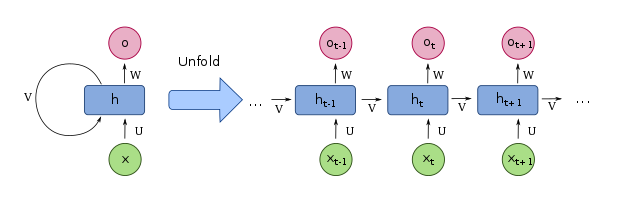
\includegraphics[width=\columnwidth]{RNN.png}
\end{center}
\begin{equation*}
    h_t = \sigma(U x_t + V h_{(t-1)} + b_h)
    \quad o_t = \text{softmax}(W h_t + b_o)
\end{equation*}
Where $ U$, $V$ and $W$ are weights matrix and the vectors $b$ are bias
parameters. Consider the gradient of $o_{t + \delta}$ with respect
to $h_t$. Applying the chain rule according to the graph above we get:

\begin{equation*}
  \nabla_{h_t} o_{t + \delta} = \left( \prod_{k = t+1}^{t+\delta} V^T
  \text{diag}(h_k(1 - h_k)) \right)\nabla_{h_{t + \delta}}o_{t + \delta}.
\end{equation*}

Thus, as $\delta$ grows, the gradient grows exponentially with $V$. If $V$ is
small or large then the gradient will either vanish or explode. A myriad
of solutions exist such as regularization through weight noise, the Long Short
Term Memory architecture tries to tackle this issue on a higher level than
regularization.
\subsection{LSTM Architecture}
To go from a RNN to a LSTM we replace hidden units with components known as
\textit{memory cells}. Our presentation and notation follows \cite{revieww}.
\begin{center}
    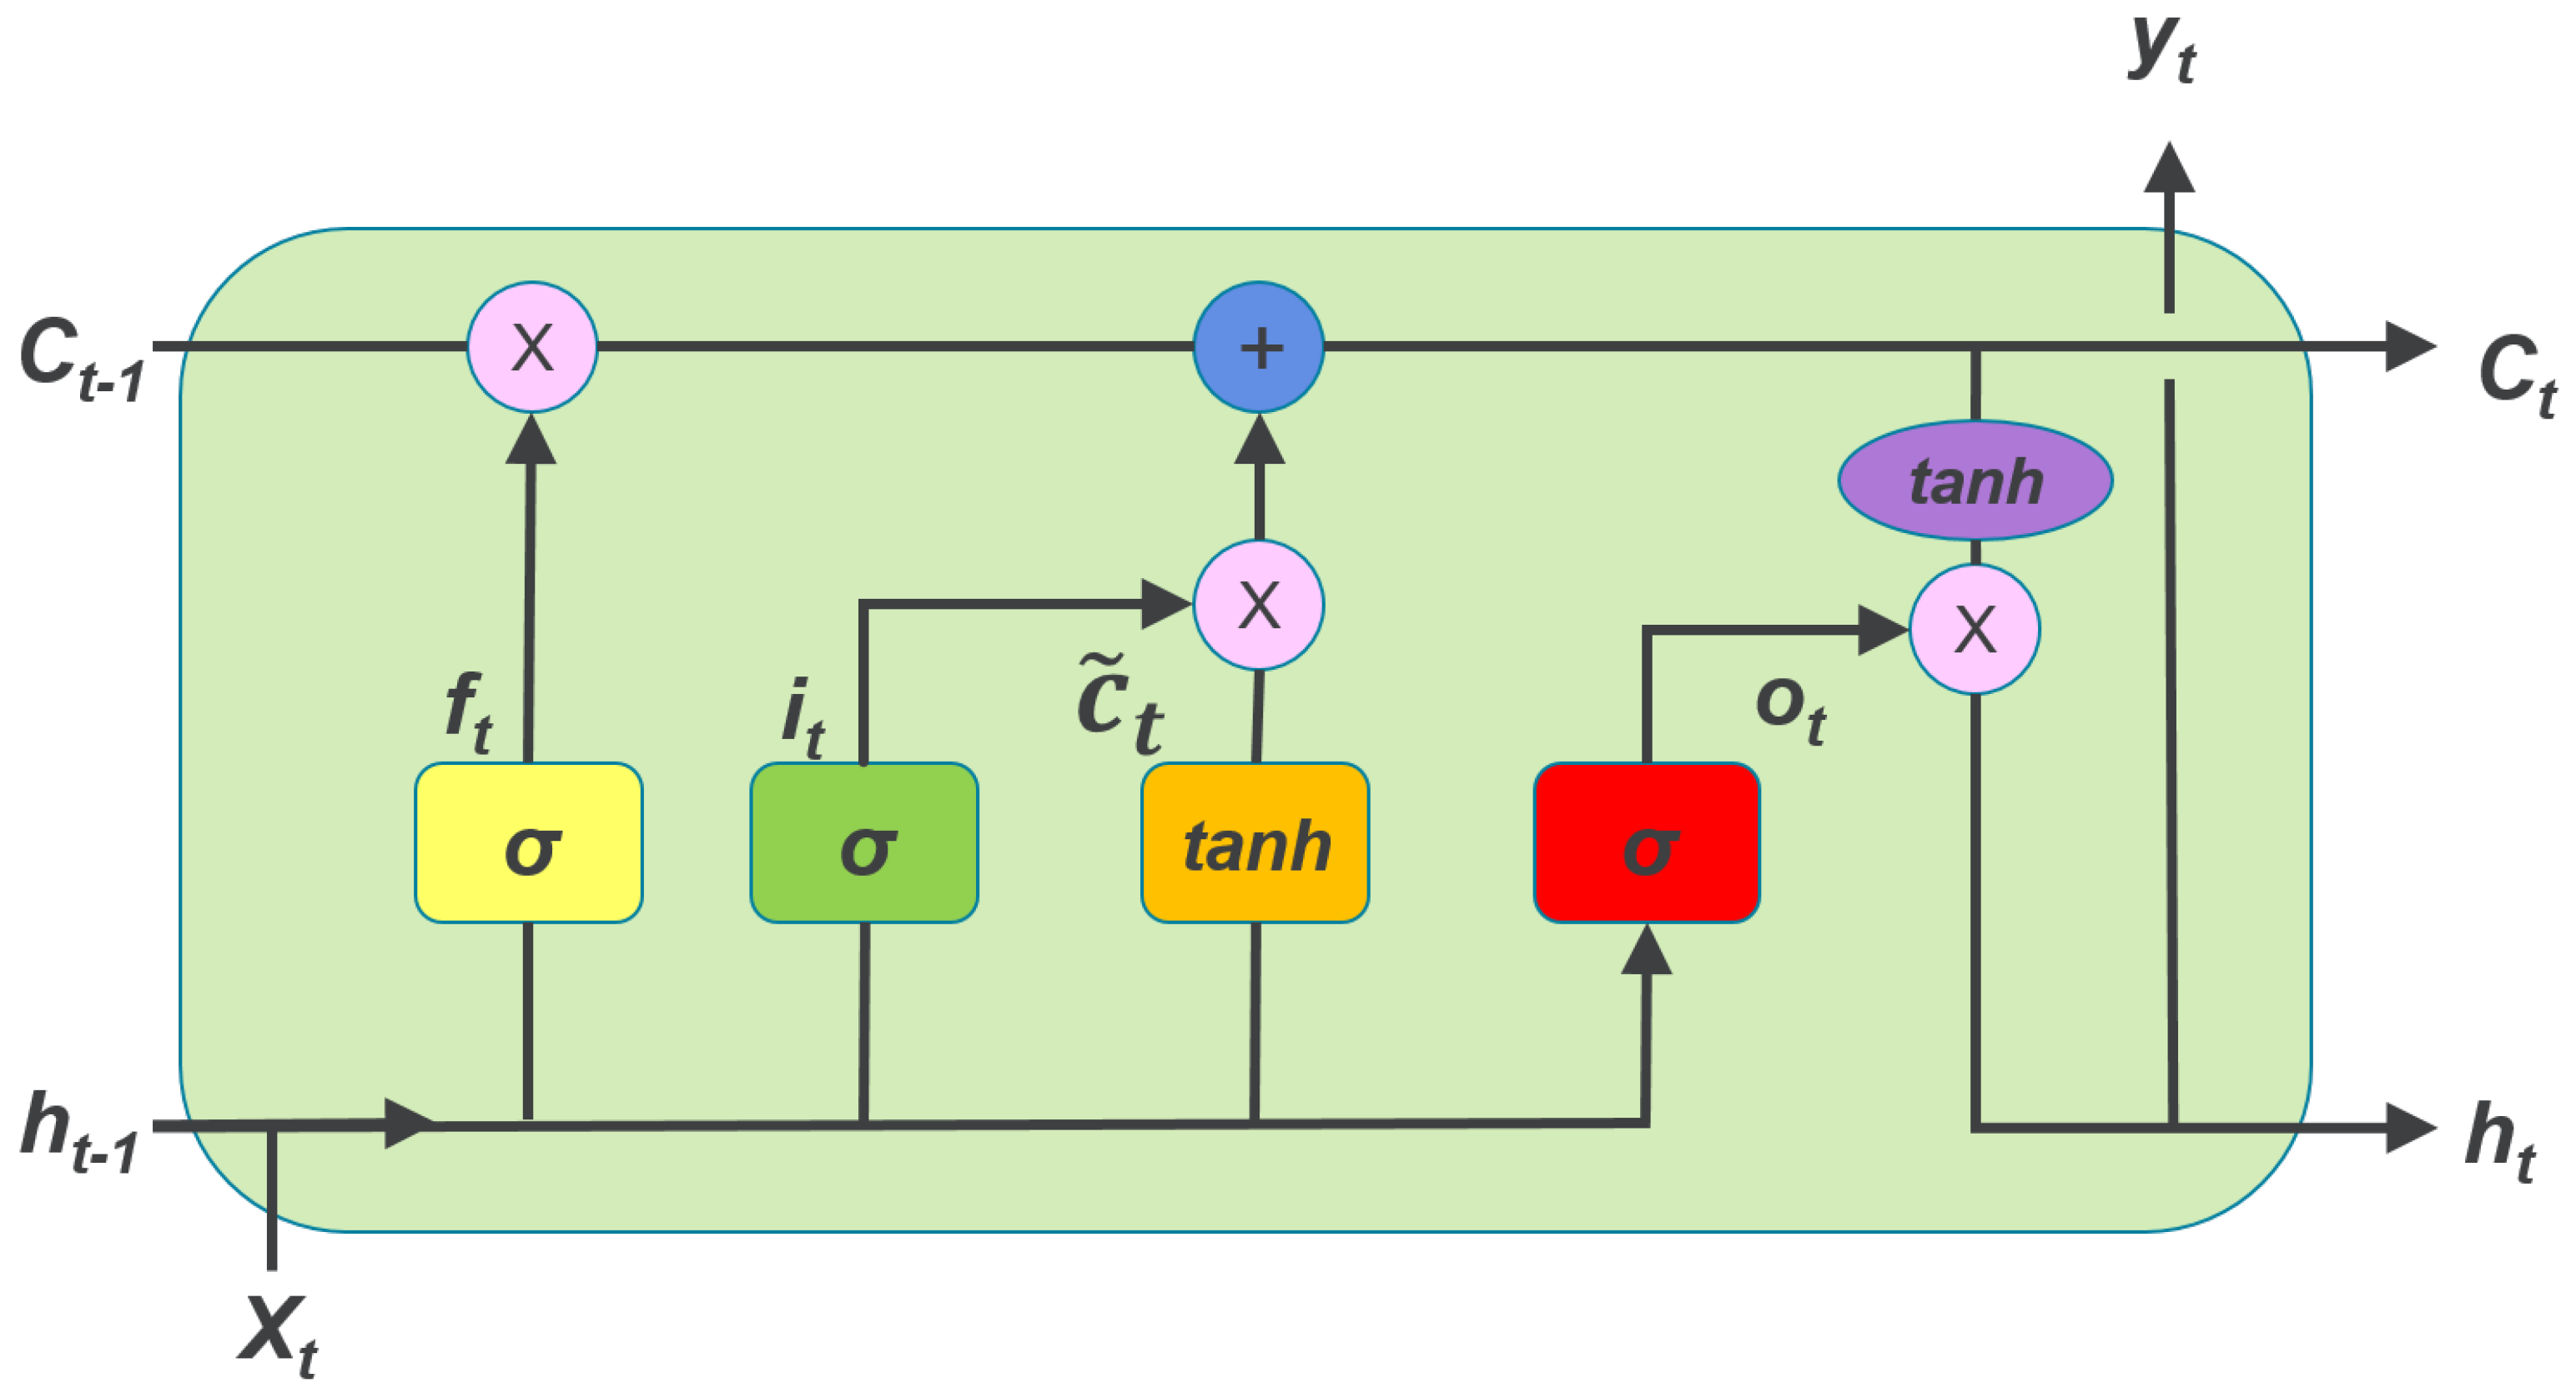
\includegraphics[width =\columnwidth]{lstm.png}
\end{center}

Intuitively, RNNs have \textit{long-term memory} in the form of matrix weights,
they change during the training; encoding through training some general
knowledge about the data. They also have \textit{short-term memory} in the form
of activation passing from each node to successive ones. The memory cell
introduced in the LSTM model formalizes those notions and provides a framework
to control their impact on the internal representation of the network.
\begin{center}
    \begin{itemize}
    \item $f_t, i_t, o_t$: Respectively forget, input and output gates.
        \begin{itemize}
            \normalsize
            \item Sigmoidal units activated through  $x_t$ (current input) and
                $h_{t-1}$ (past hidden unit output) \item $f_t$ controls the
                recursive flow
            \item $i_t$ and $o_t$ control the input and output flow
                respectively
            \item $h_t = o_t \odot \tanh(c_t)$ where $\odot$ denotes element
                wise multiplication.
        \end{itemize}
    \item $c_t = \mathbf{f_t \odot c_{t-1}} + i_t \odot \tilde{c}_t$: The cell
    which has a self-connected edge with a fixed unit weight, thereby delegating
    control of recursion to the gate
    \end{itemize}
\end{center}
The architecture of the memory cell improves the capacity to learn long time 
dependencies. Indeed, following the definition of the cell state, we have
\begin{equation*}
	c_t = \sum_{k = o}^{t}f_t \odot \dots \odot f_{k + 1} \odot i_k \odot \tilde{c}_k.
\end{equation*}
We can see that the gradient may pass over long time gaps as long as the forget 
gates are open (closed to $1$) which can be achieved with a appropriate initialization
setting a large bias  for the gates $f$. 
 
